\chapter{Introducci�n}

Debido a la creciente disponibilidad de las plataformas m�viles y el gran poder de procesamiento con el que cuentan, el n�mero de aplicaciones m�viles ha crecido de manera significativa. Dichas plataformas cuentan con sistemas de adquisici�n de audio, video y una variedad de sensores como por ejemplo aceler�metro y giroscopio, lo que las transforma en sistemas ideales para desarrollar aplicaciones de procesamiento multimedia.\\

Por otro lado, desde hace algunos a\~nos varios museos de distintas partes del mundo han comenzado a considerar este tipo de dispositivos, y otras tantas tecnolog�as, como una alternativa muy interesante para brindar un valor agregado al usuario. Proyecciones de im�genes y videos, recorridos interactivos y aplicaciones de \textit{realidad aumentada} son tan s\'olo algunos de los ejemplos. Sin embargo, esta es un �rea muy reciente y en la que todav�a queda un camino muy largo por recorrer.\\

El presente proyecto busca desarrollar sobre ciertos dispositivos m�viles en particular,  un recorrido interactivo para un museo, con realidad aumentada. Se espera de esta manera, contribuir al desarrollo de herramientas que fomenten contenidos educativos y art�sticos, generando as� un marco para poner la tecnolog�a al servicio de la cultura y la sociedad. As� entonces, se estableci� contacto con dos museos de Montevideo, el ``Museo Nacional de Artes Visuales'' (MNAV) y el ``Museo de Arte Precolombino e Ind�gena'' (MAPI). Se espera basar el prototipo final de la aplicaci�n en obras, piezas arqueol�gicas o mapas informativos, pertenecientes a estos dos museos.\\

Probablemente, la realidad aumentada sea el mayor atractivo del proyecto por ser un �rea que se encuentra en pleno desarrollo y que todo el tiempo recibe ideas innovadoras y muy interesantes, lo que la hace por dem�s apasionante. Vale la pena entonces dar una definici�n para la misma:\\

\textit{La realidad aumentada (AR del ingl�s \textit{Augmented Reality}) es un t�rmino que denota la visi�n de un entorno f�sico del mundo real, cuyos elementos se combinan con elementos virtuales generados por computadora, para la creaci�n de una realidad mixta en tiempo real.}\\

Cuando se genera una imagen por medio de realidad aumentada, conviven en ella elementos reales con elementos virtuales. Es b�sicamente un juego de percepciones. En la Figura \ref{fig: arIntro} se puede ver un ejemplo de realidad aumentada obtenido durante este proyecto. Como se puede ver se ubica un cubo virtual sobre la esquina superior izquierda del "Hombre de Vitruvio"  de manera coherente. Si en esta figura no viera el fondo, cualquier persona podr�a pensar que el cubo es real y forma parte de lo que es la obra. Esa es la intenci�n de la realidad aumentada. \\
\begin{figure}[H]
\centering
\includegraphics[scale=0.12]{figs_intro/arIntro.png}
\caption{Ejemplo de realidad aumentada. Se ubica un cubo virtual en la esquina superior izquierda de una r�plica de la obra el "Hombre de Vitruvio" de Leonardo da Vinci.}
\label{fig: arIntro}
\end{figure}

Para entender el problema de c�mo se genera la realidad aumentada primero hay que entender como se genera una imagen en una c�mara. En la Figura \ref{fig:intro_def1} se ve cual es el proceso de captura de una imagen. Se comienza por el objeto por el objeto que se quiere capturar$(1)$, luego se ubica la c�mara de manera de obtener la imagen deseada$(2)$, finalmente se captura la imagen$(3)$. 

El procedimiento para realizar la realidad aumentada se muestra en Figura \ref{fig:intro_def2}. Se comienza por la imagen de un objeto real a la cual se le quiere superponer un objeto virtual de forma coherente$(1)$. Para que el objeto real y el virtual coexistan se necesita conocer la posici�n del objeto real en el mundo$(2)$. Una vez que se conoce la posici�n del objeto real y la imagen del mismo se puede obtener la posici�n en la que estaba la c�mara cuando fue capturada esa imagen$(3)$. Una vez que se tiene la posici�n de la c�mara es posible ubicar el objeto virtual de manera coherente con el real$(4)$.

\begin{figure}[H]
\centering
\subfigure[]{
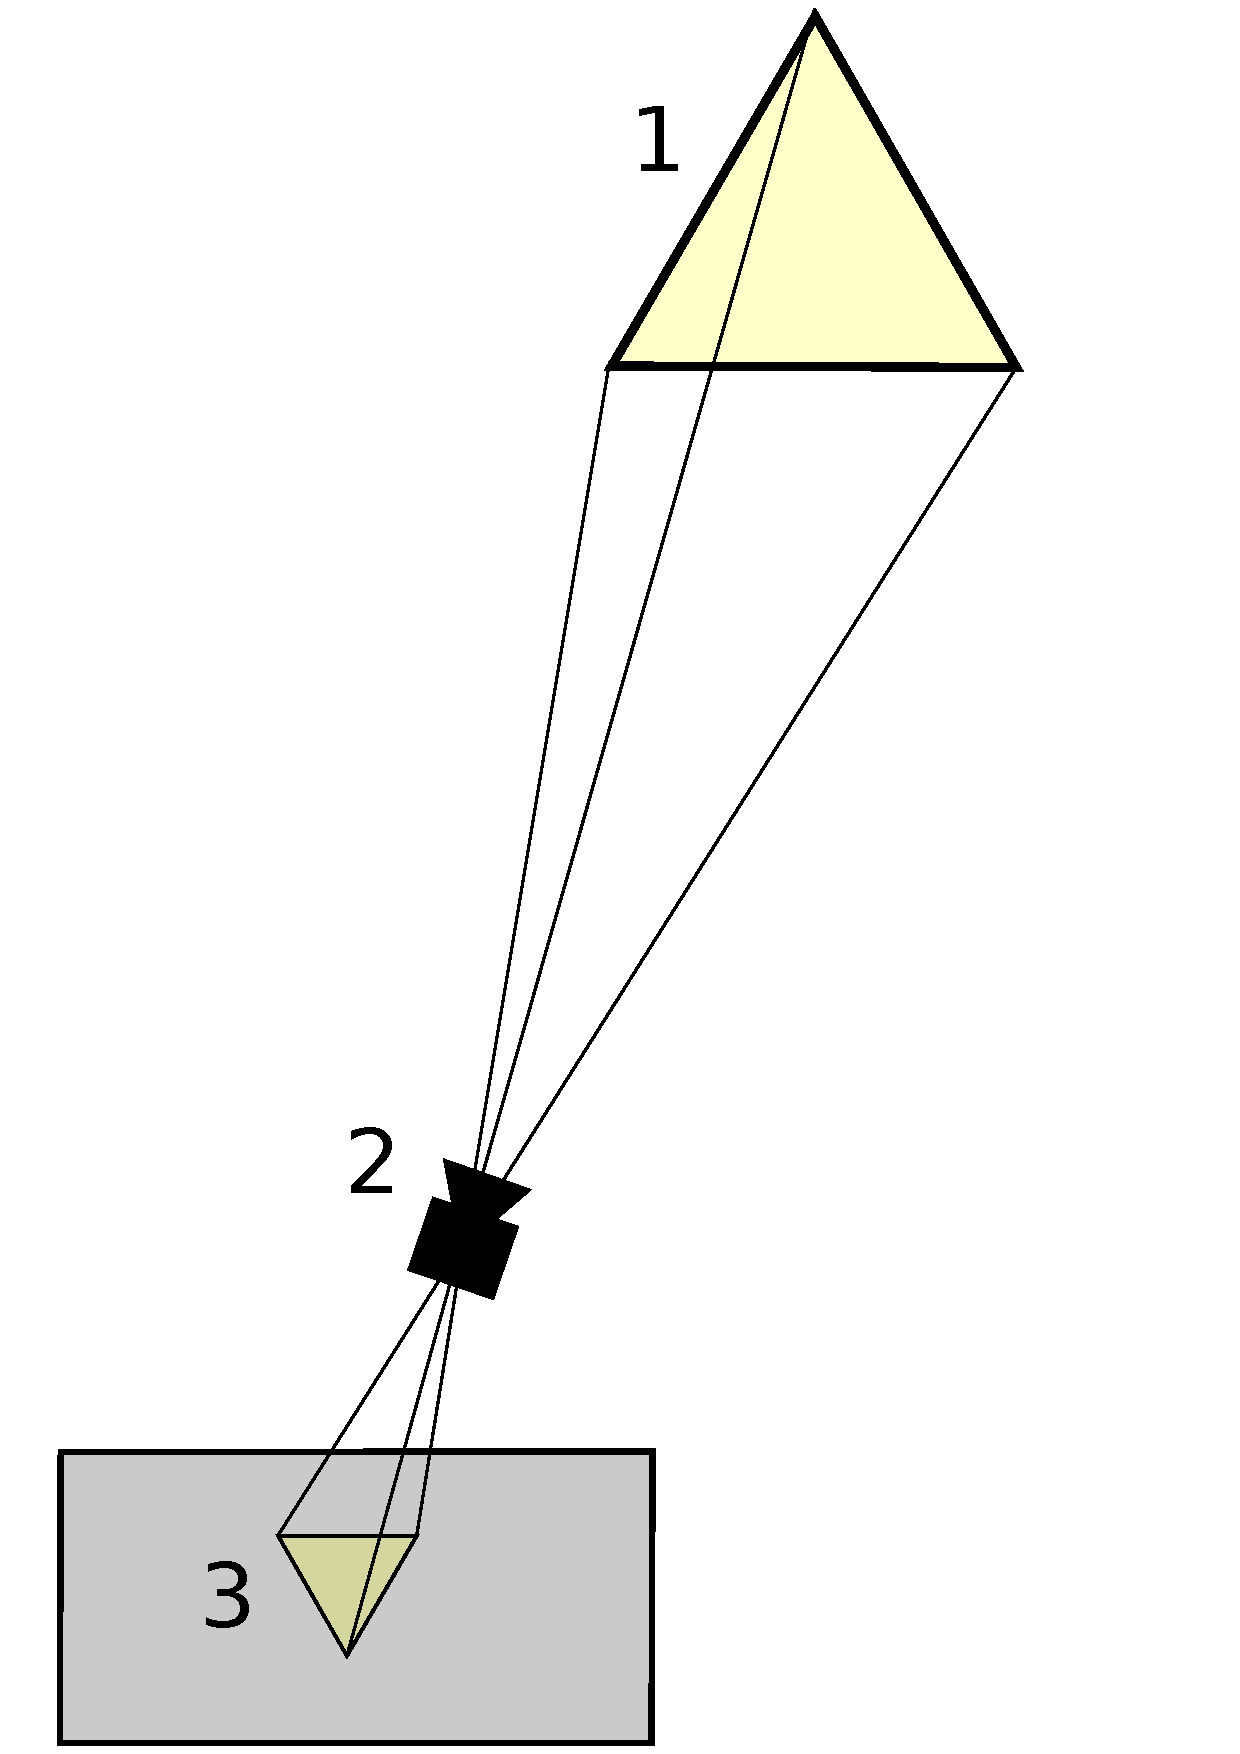
\includegraphics[scale=0.18]{figs_intro/def1}
\label{fig:intro_def1}
	}
\subfigure[]{
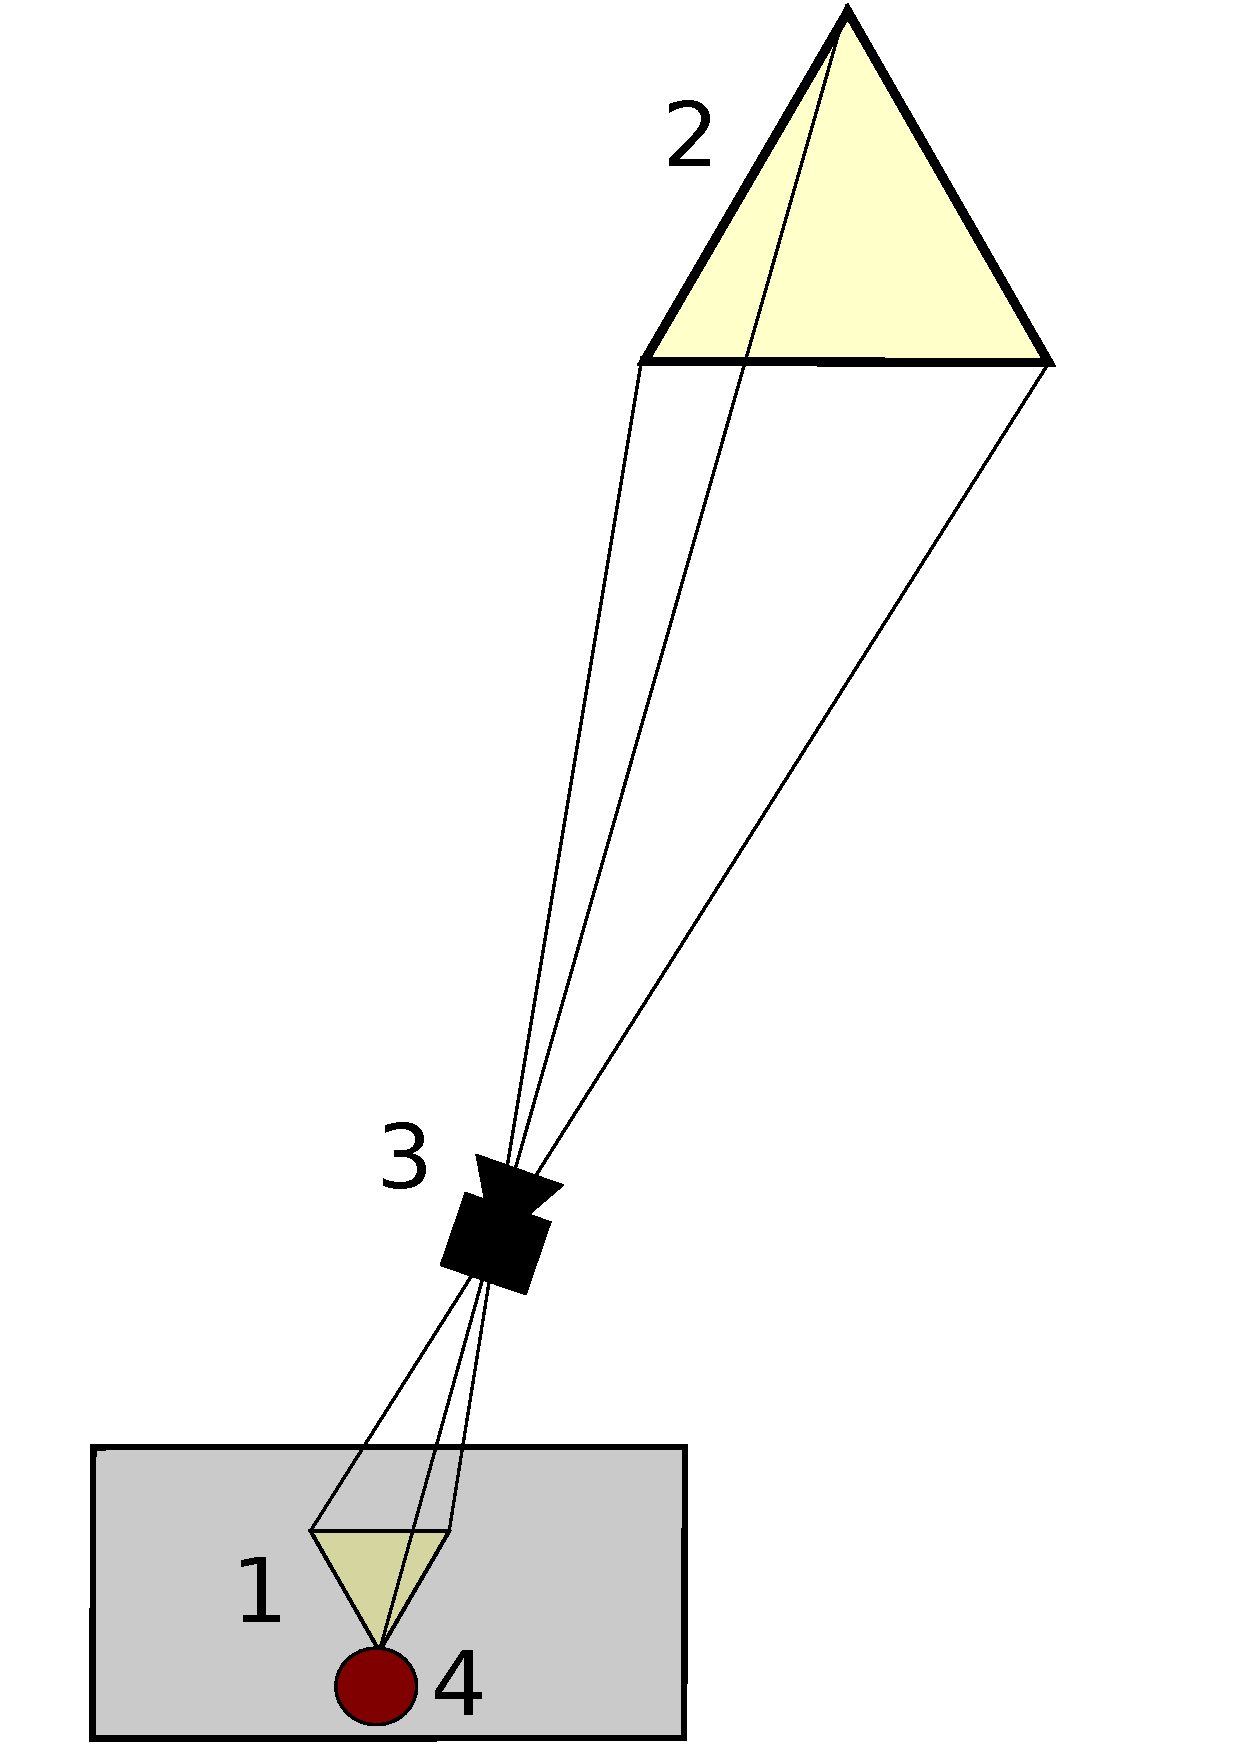
\includegraphics[scale=0.18]{figs_intro/def2}
\label{fig:intro_def2}
}
\caption{\subref{fig:intro_def1}:Pasos para capturar una imagen. \subref{fig:intro_def2}:Pasos necesarios para realizar la realidad aumentada. En ambos casos el triangulo grande es el objeto real. El objeto virtual es el circulo rojo. }
\end{figure}

A lo largo de la presente documentaci�n dar� al lector un panorama de lo que fue el proyecto en su conjunto, esperando que sirva como iniciativa para futuros trabajos vinculados a esta rama de la ingenier�a.